\documentclass[12pt]{article}
\usepackage{graphicx} % Required for inserting images
\usepackage{mathtools}
\usepackage{amsmath}
\usepackage{gvv-book}
\usepackage{gvv}
\usepackage[shortlabels]{enumitem}
\usepackage{multicol}

\title{\textbf{10.3.2}}
\author{\textbf{EE25BTECH11004 - Aditya Appana}}
\date{October 4, 2025}
\renewcommand{\labelenumi}{\Alph{enumi})}
\begin{document}

\maketitle

\section*{Question}
Prove that the curves $y^2 = 4x$ and $x^2 + y^2-6x + 1 = 0$ touch each other at the point (1,2).
\section*{Solution}
To solve this question, we need to find the tangent at the given point to each of the curves. We can then prove that the curves touch each other at the point \textbf{if both tangent equations are the same}.\\
$y^2 = 4x$ and $x^2 + y^2-6x + 1 = 0$ represented in the form \setcounter{equation}{-1} \begin{align}\vec{x^T}\vec{V}\vec{x} + 2\vec{u^T}\vec{x}+f = 0\end{align} are:

\begin{align}
    \vec{x}^T\myvec{0&0\\0&1}\vec{x} + 2\myvec{-2\\0}^T\vec{x} = 0
\end{align}
and
\begin{align}
    \vec{x^T}\myvec{1&0\\0&1}\vec{x} + 2\myvec{-3\\0}^T\vec{x} + 1 = 0
\end{align}
respectively.\\
Given the point of contact $\vec{q}$, the equation of tangent to (1) is:
\begin{align}
    \brak{\vec{Vq} + \vec{u}}^T\vec{x} + \vec{u}^T\vec{q} + f = 0
\end{align}
Therefore, the tangent to (1) at $\myvec{1\\2}$ is:
\begin{align}
    \brak{\myvec{0&0\\0&1}\myvec{1\\2} + \myvec{-2\\0}}^T\vec{x} + \myvec{-2\\0}^T\myvec{1\\2} = 0\\
    \myvec{-2\\2}^T\vec{x} - 2 = 0
\end{align}\\
The tangent to (2) at $\myvec{1\\2}$ is:
\begin{align}
    \brak{\myvec{1&0\\0&1}\myvec{1\\2} + \myvec{-3\\0}}^T\vec{x} + \myvec{-3\\0}^T\myvec{1\\2} + 1 =0\\
    \myvec{-2\\2}^T\vec{x} - 2 = 0
\end{align}\\
Both equations are the same, \textbf{hence proved}.

\begin{figure}[H]
    \centering
    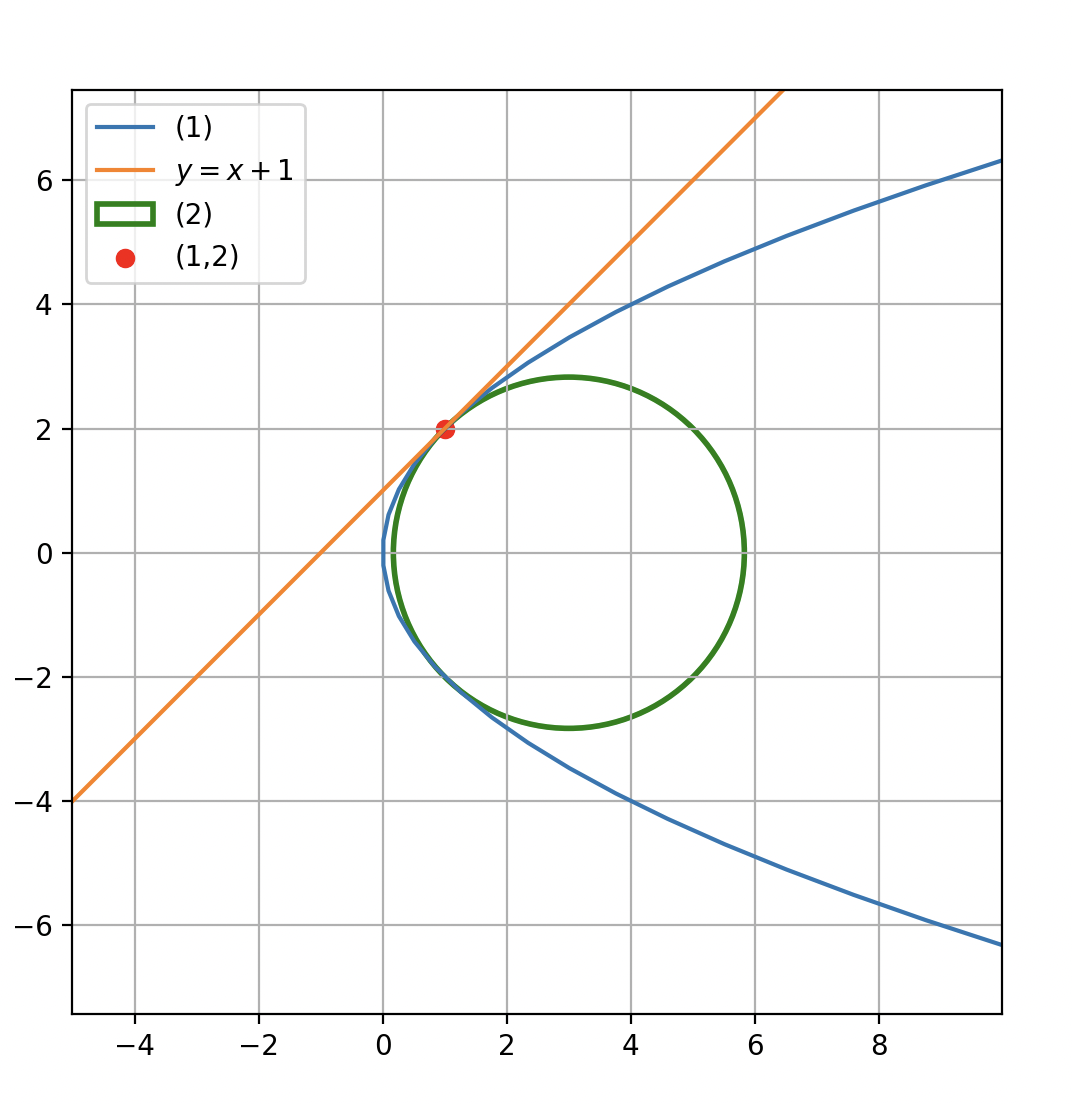
\includegraphics[width=0.9\columnwidth]{Figs/1032.png}
    \caption{Plot}
    \label{fig:placeholder}
\end{figure}
\end{document}